% !TEX root = ../../../../main/numb3rs_activities.tex
\newpage
\phantomsection
\addcontentsline{toc}{subsection}{109: Sniper Zero  \label{ep109}}
\ep{109: Sniper Zero}
\setcounter{activity}{0}


In this episode the FBI investigates a bizarre string of sniper attacks which seem to have little in common. To determine the location of the sniper in each shooting, Charlie uses ballistic trajectory modeling. Exponential growth and regression to the mean are also briefly mentioned, and the first of these we explore in depth below.


% Ballistic
\ltLarge{Ballistic Trajectory}


A bullet, like any other object flying through the air, is subject to the forces of gravity, air resistance, and wind. One way to closely approximate the actual trajectory is to ignore the effects of drag and wind, instead looking only at gravity.

	\begin{figure}[H] 
	\centering
	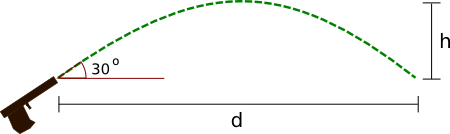
\includegraphics[width=0.75\textwidth]{../sections/seasons/season1/109/images/109(1).png} 
	\end{figure}
	
Consider the figure above. A bullet leaves the barrel of a gun inclined at a $30^\circ$ angle and flies a horizontal distance of d before reaching the starting elevation. The force of gravity acts on the bullet, creating a downward acceleration of $g= 9.8~\text{m}/\text{sec}^2$ and so influencing the vertical component of the velocity vector (see diagram below) over time. Since we disregard drag, the horizontal component of the velocity does not change.

	\begin{figure}[H] 
	\centering
	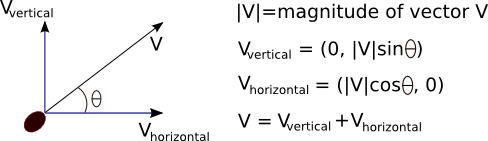
\includegraphics[width=0.75\textwidth]{../sections/seasons/season1/109/images/109(2).png} 
	\end{figure}

The next activity involves figuring out the equations describing the speed and position of an object in free-fall. These derivations make some use of \bref{calculus}{https://en.wikipedia.org/wiki/Calculus}. Try to follow them and do the exercises, but if you can't, just use the equations mentioned in order to do Activity 2.


\tangent{Technically, the term \emph{velocity} means the vector pointing in the direction of motion with magnitude equal to the \emph{speed} of the object. However, in everyday usage and even in many physics textbooks the term velocity is used to denote both the vector and its magnitude, the speed. It is usually easy to figure out which is being meant from the context: just ask yourself, is the sentence talking about a vector or a scalar?}


\activity{Let us first consider only the vertical direction of motion. For the sake of brevity, I'll just write $v(t)$ below instead of $v_{\text{vertical}}(t)$.
\begin{enumerate}[1.]
\item Recall that the acceleration of an object is equal to the instantaneous change in velocity, i.e. $a(t)=v'(t)$. Apply the \bref{fundamental theorem of calculus}{https://en.wikipedia.org/wiki/Fundamental_theorem_of_calculus} to this equality to deduce that $v(t)-v(0)=gt$, where $g$ is the acceleration due to gravity.
\item We can do even better by applying the same trick to velocity. Namely, we know that $v(t)=y'(t)$, where $y(t)$ is the vertical position of the object at time $t$. Apply the fundamental theorem of calculus again to show that 
	\[
	y(t)=y(0)+v(0)t+\frac{gt^2}{2}
	\]
\item Now write down an equation for the horizontal position $x(t)$ of the bullet in terms of the initial horizontal velocity $v_{\text{horizontal}}(0)$. (Hint: remember, we disregard drag and wind so the only acting force is gravity.)
\end{enumerate}
}


\activity{\label{act:109_2}%
Suppose the bullet is fired at an angle of $30^\circ$ as in the first picture, with a speed of 900m/s from an initial point $x(0)=0$ and $y(0)=0$ (i.e. from the origin) at time $t=0$. Use the equations from activity 1 to answer the following questions.
\begin{enumerate}[1.]
\item What is the maximum height achieved by the bullet? At what time is this height achieved? [Hint: what is the vertical velocity of the bullet when it's at a peak height?]
\item What is the horizontal distance of the bullet from the origin at the time of peak height? What is the distance to the point at which the bullet is again at the height from which it was fired; that is, $y= 0$?
\item Show that the trajectory of the bullet is a \bref{parabola}{https://en.wikipedia.org/wiki/Parabola}.
\end{enumerate}
}


Analyzing the general situation, in which both wind and drag affect the path of a bullet, is in fact very complicated. You can get a taste of the difficulties involved by reading the wikipedia article on \bref{external ballistics}{https://en.wikipedia.org/wiki/External_ballistics}. Furthermore, mathematically recreating the path of a bullet after it has hit a target, thus only knowing its angle of entry, is much harder.


% Exp Growth
\ltLarge{Exponential Growth}


Here are a few recent uses of the term exponential growth in the news media:


The company has had a spectacular two years, riding the exponential growth in oil prices that helped to increase profits by a fifth in 2006 to \pounds 28.5 million. (\emph{Business Big Shot: Alasdair Locke}, The Times, Dec 20, 2007)


After years of exponential growth, there has recently been a slow down in the Northern Ireland property market. (\emph{Well-known property firms merge}, BBC News, Dec 7, 2007)


Kessler himself came under university scrutiny for alleged financial irregularities. In January 2005, an anonymous source contended he ``spent or formally committed all of the reserves of the dean's office and has also incurred substantial long-term debt in the form of lavish salary increases and exponential growth in new, highly compensated faculty and staff directly reporting to him." (\emph{UCSF dean is fired, cites whistle-blowing}, Los Angeles Times, Dec 15, 2007)


While the above excerpts describe growth in entirely different areas, the one thing they have in common is the use of the term \emph{exponential growth}. In mathematics, we say that quantity $x$ grows exponentially with respect to time $t$ if $x$ satisfies the following differential equation: $\frac{dx}{dt}=kx$, where $k$ is a constant and $\frac{dx}{dt}$ is either a derivative, when $t$ is continuous, or the change in $x$ in a given time interval, when $t$ is discrete. In plain words, this means that $x$ grows exponentially if it increases proportionally to its own value. Most often exponential growth occurs in situations where ``$x$ creates more $x$", typical examples being population growth and compound interest. Exponential growth can occur both when the time intervals are discrete, for example in annual or monthly interest compounding, and when the time variable is continuous, as in continuous compounding of interest or modeling of large populations. The discrete time case is more often encountered in practice and is easier to analyze mathematically, since we don't need to resort to the exponential function.


\activity{
\begin{enumerate}[1.]
\item Suppose yesterday you heard that annual inflation was 3\% in the last year. If $x$ is the price of a representative \bref{basket of goods}{https://en.wikipedia.org/wiki/Market_basket}, and $t$ is measured in years, what is the corresponding proportionality constant $k$ in the exponential growth equation that models the price increase? (Hint: note that in this case $dt=1$ year.)
\item What if $t$ is measured in days instead?
\end{enumerate}
}


The reason why such growth is called exponential is that when the time variable $t$ is continuous, we can solve the differential equation $\frac{dx}{dt}= kx$. By separating variables we get $\frac{dx}{x}= k\;dt$, integrating we arrive at $\ln(x)= kt + C$, where $C$ is some constant, and exponentiating both sides, we finally get $x= D\,e^{kt}$, where $D$ is a constant. We can solve for $D$ by plugging in $t= 0$, the starting time, to arrive at the general solution $x(t)= x(0)\,e^{kt}$. Exponential growth is much faster than polynomial, as the example below illustrates in case of $e^t$ versus $t^3$. \\

	\begin{figure}[H]
	\centering
	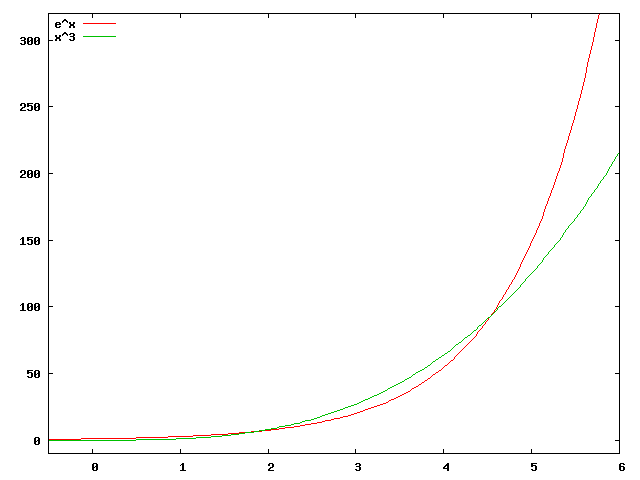
\includegraphics[width=0.75\textwidth]{../sections/seasons/season1/109/images/109e8.png} 
	\end{figure}


\activity{
\begin{enumerate}[1.]
\item Find a constant $r$ so that $2^t= e^{rt}$.
\item Show that $2^t$ becomes larger than any polynomial in $t$, for sufficiently large $t$. (Hint: suppose $p(t)= t^n$ for some positive integer $n$. For which $t$ is $2t > p(t)$?)
\item Can you think of a function $f(t)$ which grows faster than an exponential function, in the sense of part 2 above?
\end{enumerate}
}


In practice, when talking about compound interest two quantities are important. One is the annual interest rate, sometimes called the annual percentage rate (APR). The other is the number of compounding periods per year: how many times per year is the interest added to the principal amount. For instance, say you have \$100 credit card debt with an APR of 20\%. Usually credit cards compound monthly, so there are 12 compounding periods per year. Thus if you make no payments (and incur no additional penalties or expenses) for a whole year, your debt will \emph{not} simply be $100 + 100 \cdot 0.2= 120$, which it would if the interest was compounded \emph{only once per year}. Instead, after the first month, you'll owe $100 + 100 \cdot \left( \frac{0.2}{12} \right) = 101.67$ dollars. After the second month, you'll owe $101.67 + 101.67 \cdot \left( \frac{0.2}{12} \right)= 103.36$ dollars, and so on. At the end of the year, with such monthly compounding, you'll owe \$121.94. Might not seem like a huge difference from the once a year compounding sum of \$120, but over longer periods of time, the difference becomes substantial.


\activity{
\begin{enumerate}[1.]
\item You open a savings account which earns 2\% interest with a deposit of \$1000. Would you rather the interest compound daily or monthly? Write down the formula for the amount of money in the account after a year in both cases. (Hint: write down the expression for the amount of money after one period of compounding, now after two periods (don't simplify!), then three... See the pattern?)
\item Suppose we decide to compound not once a month or a day, but once every split second. In fact, we can let the number of compounding periods go to infinity, thus letting the length of each period approach zero. Use the fact that $e^y= \lim_{n \to \infty} \left(1 + \frac{y}{n} \right)^n$, for any real number $y$, to show that when the number of compounding intervals goes to infinity, then after $t$ years, your account will have $1000 e^{0.02t}$ dollars. This is continuous compounding.
\end{enumerate}
}


\activity{In popular usage, the expression ``exponential growth" is often used as a synonym for ``very fast growth". There's no good reason to describe faculty hiring practices, as the third quote in the beginning of this section does, in terms of exponential growth. While an exceptional number of faculty might have been added during Kessler's tenure as dean, there's no sense in which ``faculty makes more faculty" proportionally to existing numbers. At other times, ``exponential growth" can be more accurately described as \bref{sigmoidal}{https://en.wikipedia.org/wiki/Sigmoid_function} (remember that strange function used in \hyperref[ep218]{logistical regression}?). While similar in the low range to the exponential function, sigmoidal growth reflects the fact that at some point growth must slow down due to lack of resources.}